\chapter{Funktionale Anforderungen}

\section{\gls{App}}
\begin{enumerate}
\renewcommand{\labelenumi}{\textbf{\theenumi}}
\renewcommand{\theenumi}{FA\arabic{enumi}0}
\setcounter{enumi}{99}
\item \label{fa:anmeldeAnsicht} \textbf{Anzeigen der Anmeldeansicht} \hfill \\
Öffnet der Benutzer die \gls{App} und sind keine Nutzerdaten gespeichert~\eqref{fa:loginApp}, so gelangt er in die Anmeldeansicht, in der er sich anmelden kann. Das Erstellen von Benutzeraccounts ist hier \textbf{nicht} möglich.

\item \label{fa:Anmeldedaten}\textbf{Anmeldedaten speichern} \hfill \\
Anmeldedaten bestehen aus der E-Mail-Adresse und dem Passwort des Nutzers und werden lokal auf dem Gerät abgespeichert. Das Passwort wird als \gls{Hash-Code} gespeichert.

\item \label{fa:loginApp} \textbf{Anmelden in der \gls{App}} \hfill \\
Beim Appstart muss sich der Nutzer zunächst anmelden. Zum Anmelden müssen die Anmeldedaten~\eqref{fa:Anmeldedaten} des Nutzers korrekt in die entsprechenden Felder eingetragen sein. Nur verifizierte Nutzer~\eqref{fa:erstellAcc} können sich anmelden. Bei falschen Eingaben erhält der Nutzer eine Fehlermeldung. Hat sich ein Nutzer bereits zuvor angemeldet, ohne sich wieder abzumelden, gelangt der Nutzer direkt zur Kamera-Ansicht. Die Überprüfung der gespeicherten Anmeldedaten erfolgt erst beim Hochladen von Videodaten auf den Server~\eqref{fa:vidHochladen}.

\item \label{fa:logOut}\textbf{Abmelden von einem Benutzeraccount} \hfill \\
Klickt ein Benutzer im Menü auf ``abmelden'', so wird er auf die Anmeldeansicht~\eqref{fa:anmeldeAnsicht} geleitet und seine lokalen Anmeldedaten~\eqref{fa:Anmeldedaten} vom Gerät gelöscht.

\item \label{fa:Beobachtungsmodus}\textbf{Ausführen des Beobachtungsmodus} \hfill \\
Die Kamera kann sich bei aktiver Kamera in zwei Modi befinden: Im Beobachtungsmodus oder im Aufnahmemodus~\eqref{fa:Aufnahmemodus}.
Im Beobachtungsmodus werden Kamerabilder nicht persistiert ~\eqref{fa:Persistieren} sondern nur der \gls{Ringpuffer}~\eqref{fa:Ringpuffer} beschrieben. Die \gls{G-Sensor}-Daten werden ausgewertet und es wird auf einen charakteristischen Ausschlag des G-Sensors ~\eqref{fa:automUebergang}, oder manuelles Auslösen ~\eqref{fa:manUebergang} gewartet.

\item \label{fa:Statussymbol}\textbf{Anzeigen des Statussymbols} \hfill \\
Der aktuelle Kameramodus wird dem Nutzer durch ein blinkendes Statussymbol am Bildschirmrand visualisiert. Im Beobachtungsmodus hat es eine grüne Farbe, im Aufnahmemodus hat es eine rote Farbe.

\item \textbf{Stoppen der Beobachtung} \hfill \\
Wenn der Benutzer die Kamera-Ansicht ~\eqref{fa:kamAnsicht} während der Beobachtung verlässt, oder die \gls{App} schließt, wird die Beobachtung automatisch beendet.

\item \label{fa:automUebergang}\textbf{Durch \gls{G-Sensor} ausgelöster Übergang in den Aufnahmemodus} \hfill \\
Werden die in~\eqref{na:GSensfront} -~\eqref{na:GSensvert} definierten Richtwerte des G-Sensors überschritten, während die \gls{App} die Kamera-Ansicht~\eqref{fa:kamAnsicht} anzeigt, geht die Kamera in den Aufnahmemodus über~\eqref{fa:Aufnahmemodus}. 

\item \label{fa:manUebergang}\textbf{Manueller Übergang in den Aufnahmemodus} \hfill \\
Befindet sich die Kamera im Beobachtungsmodus~\eqref{fa:Beobachtungsmodus}, geht sie nach doppeltem Tippen auf die Vorschaufläche der Kamera-Ansicht~\eqref{fa:kamAnsicht} in den Aufnahmemodus ~\eqref{fa:Aufnahmemodus} über.

\item \label{fa:Aufnahmemodus}\textbf{Ausführen des Aufnahmemodus} \hfill \\
Im Aufnahmemodus wird der \gls{Ringpuffer} zunächst für 30 Sekunden beschrieben ~\eqref{fa:Ringpuffer}und anschließend der komplette Inhalt des Puffers im Hintergrund persistiert~\eqref{fa:Persistieren}. Weitere \gls{G-Sensor}-Ausschläge, sowie Nutzereingaben werden während sich die Kamera im Aufnahmemodus befindet ignoriert. Die Messwerte des G-Sensors, Zeit und Auslöseart (\eqref{fa:automUebergang}, ~\eqref{fa:manUebergang}) werden in die \gls{Metadaten} der Videodatei geschrieben. Nach Ablauf der erwähnten 30 Sekunden wechselt die Kamera wieder zurück in den Beobachtungsmodus~\eqref{fa:Beobachtungsmodus}.

\item \label{fa:Ringpuffer}\textbf{\gls{Ringpuffer} beschreiben} \hfill \\
Im Beobachtungsmodus ~\eqref{fa:Beobachtungsmodus} wird der \gls{Ringpuffer} mit den Videodaten der Kamera beschrieben. Die Tonspur wird verworfen. Die auf dem Ringpuffer vorhandenen Daten sind nicht verschlüsselt und daher dem Benutzer auch nicht zugänglich. Der Ringpuffer hält bis zu einer Minute Videomaterial ~\eqref{na:Ringpuffer}.

\item \label{fa:Persistieren}\textbf{Video \gls{persistieren}} \hfill \\
Beim Persistieren, werden die Videodaten zunächst verschlüsselt~\eqref{fa:Verschluesselung} und daraufhin auf dem internen Speicher hinterlegt.

\item \label{fa:Verschluesselung}\textbf{Verschlüsseln eines Videos} \hfill \\
Dem Nutzer zugängliche Videodaten werden durch das unter~\ref{sec:Verschlüsselung} beschriebene hybride Verschlüsselungsverfahren verschlüsselt.

\item \begin{minipage}[t]{\linewidth} 
\textbf{Anzeigen des Menüs} \hfill \\
	\begin{wrapfigure}{r}{0.4\linewidth}
		\vspace{-70pt}
  		\begin{center}
   			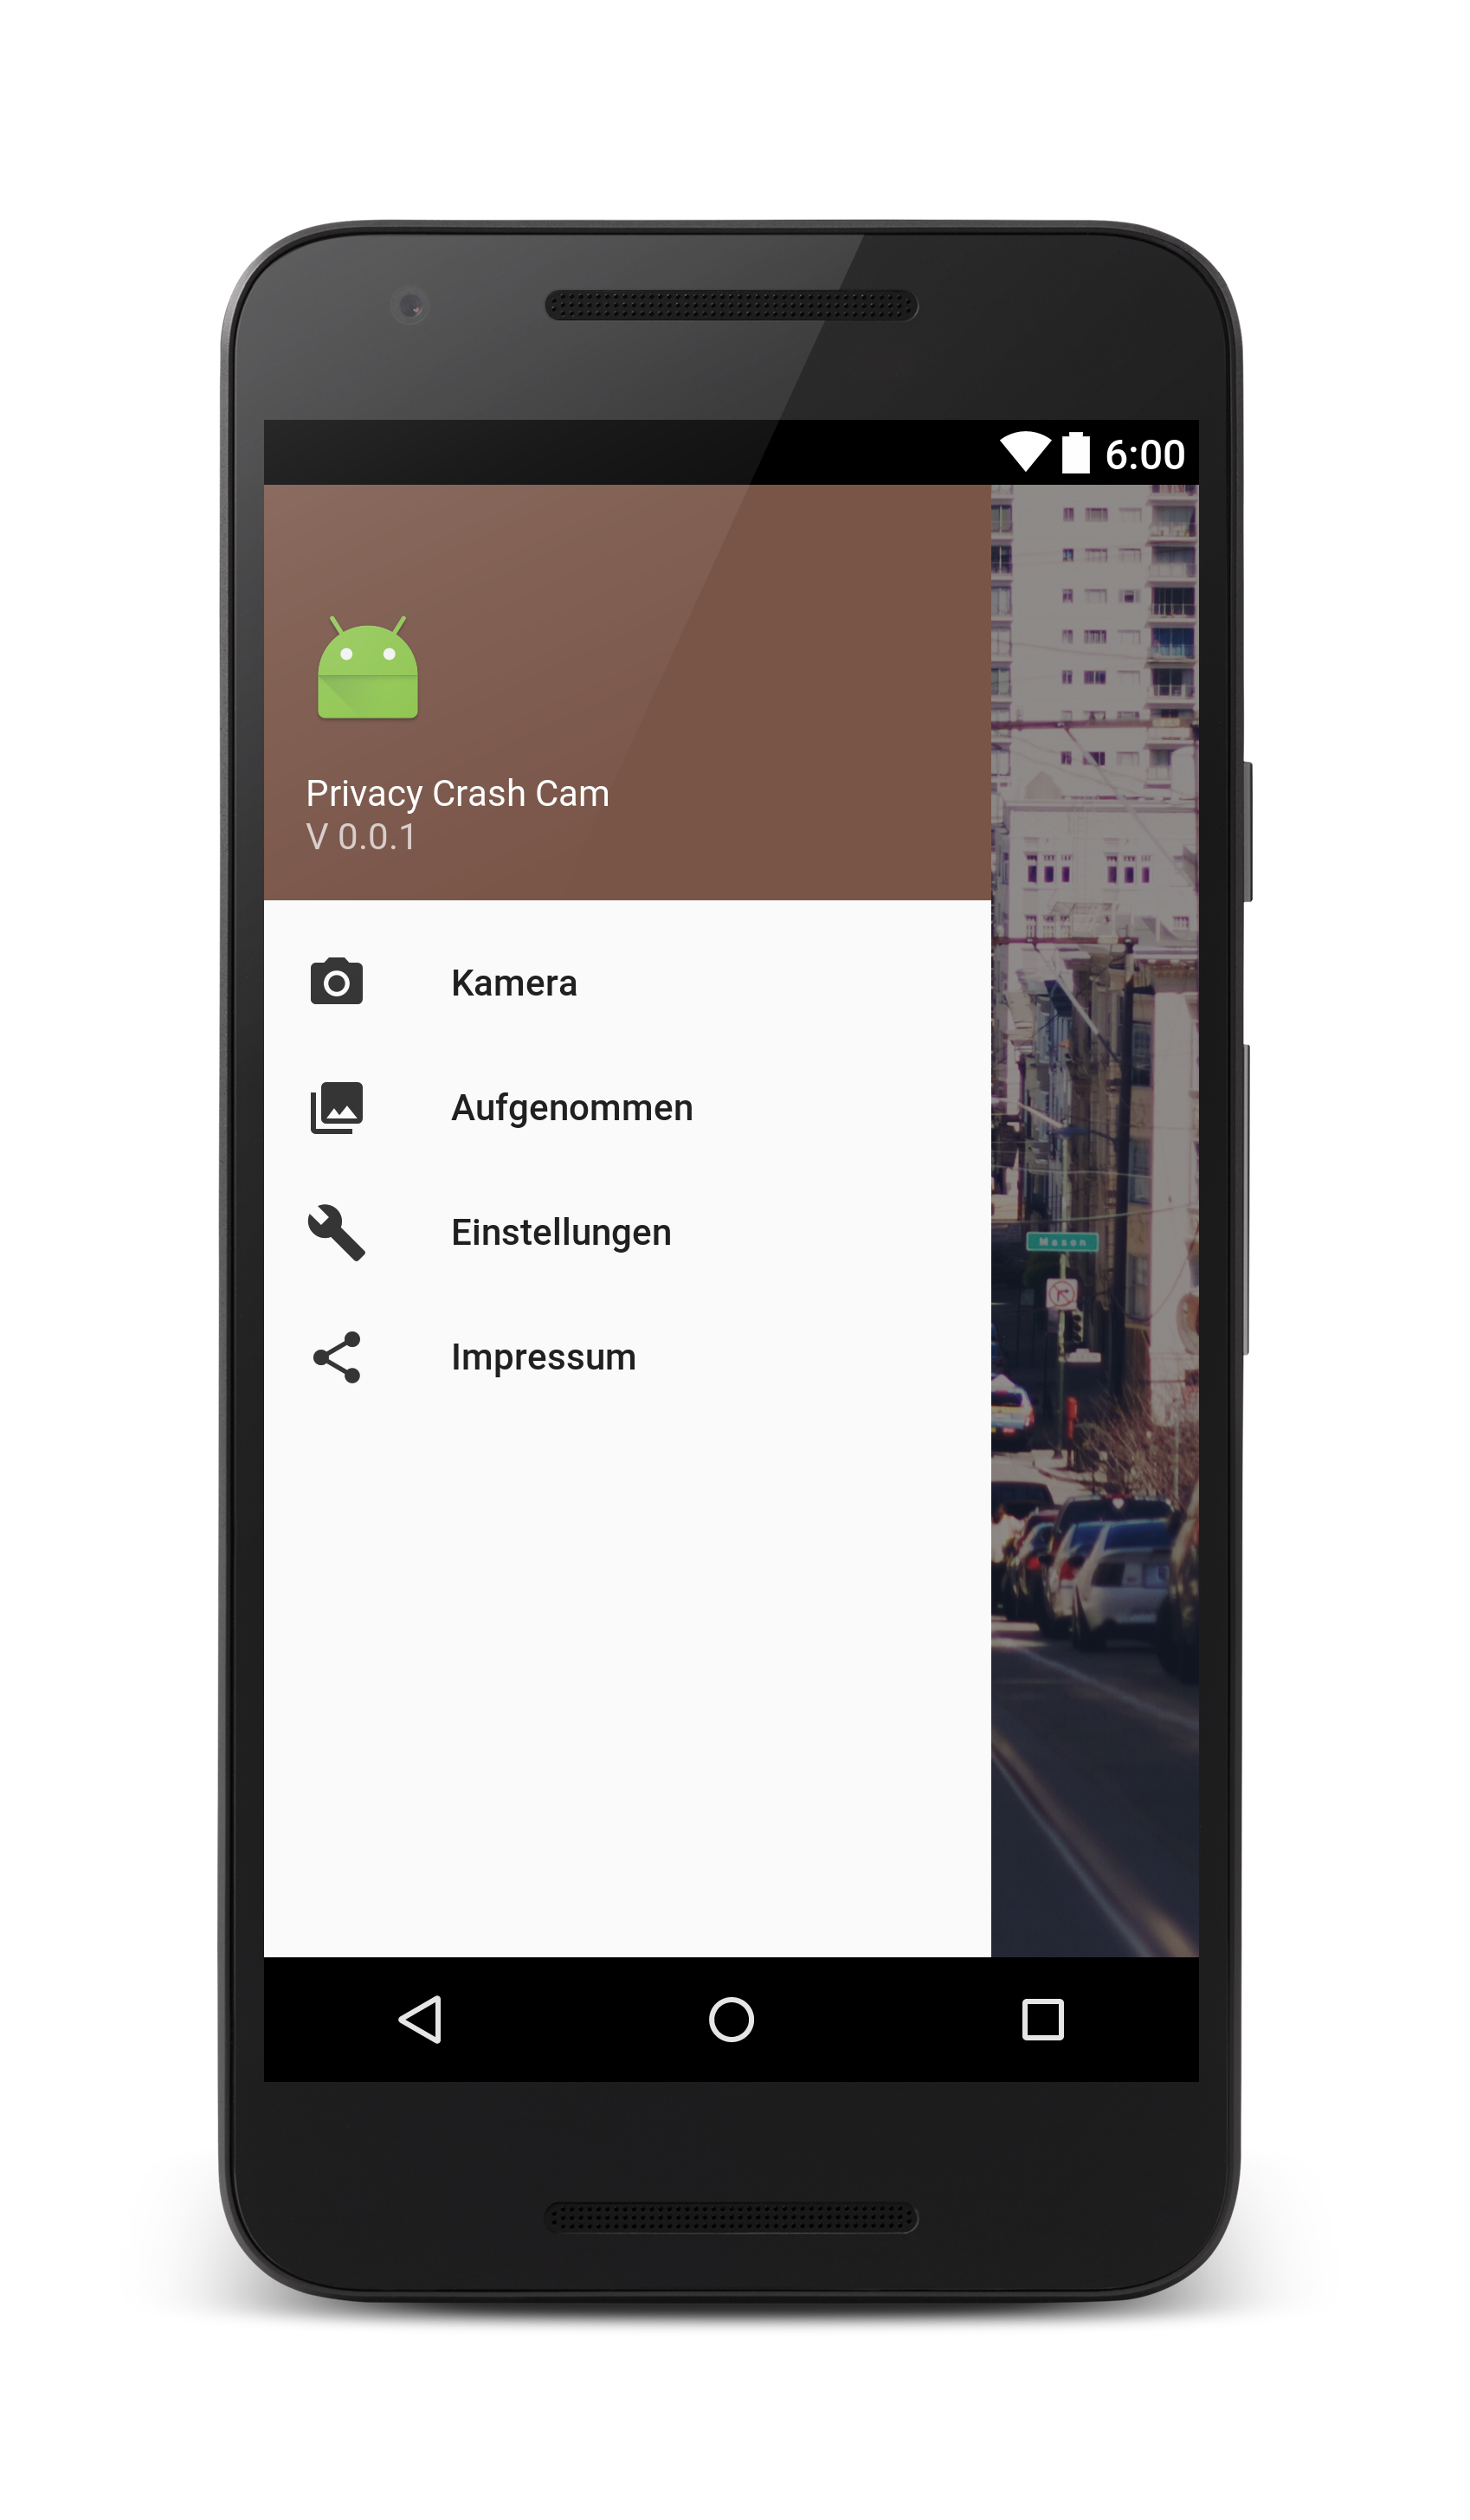
\includegraphics[width=0.4\textwidth]{subtopicsFuncspec/Res/Mockups/Portrait_camera_view_menu_phone.png}
  		\end{center}
  		\vspace{-20pt}
  		\vspace{-10pt}
	\end{wrapfigure}
Drückt der Benutzer den ``Menü-Button'' in der oberen linken Ecke des Bildschirms, so öffnet sich das Menü. Wenn sich die Kamera im Beobachtungsmodus befindet, während das Menü geöffnet wird, wird die Aufnahme nicht gestoppt. In dem Menü hat der Benutzer die Möglichkeit zwischen den verschiedenen \gls{App}-Ansichten Kamera-Ansicht~\eqref{fa:kamAnsicht}, Liste der persistierten Videos~\eqref{fa:vidAnsicht}, Einstellungs-Ansicht~\eqref{fa:einstAnsicht} und Impressum-Ansicht~\eqref{fa:imprAnsicht} zu wählen, oder sich abzumelden~\eqref{fa:logOut}.

\item \label{fa:kamAnsicht}\textbf{Anzeigen der Kamera-Ansicht} \hfill \\
Wenn sich ein Benutzer gerade angemeldet hat oder im Menü die Option ``Kamera'' wählt, so gelangt er zur Kamera-Ansicht. Dort sieht er die Vorschau seines Kamerabildes. Zudem gelangt er automatisch in den Beobachtungsmodus~\eqref{fa:Beobachtungsmodus}.

\item \label{fa:vidAnsicht}\textbf{Anzeigen der Liste der \glslink{persistieren}{persistierten} Videos} \hfill \\
Wählt der Benutzer im Menü die Option ``Videos'', so gelangt er zu einer Ansicht, in dem ihm seine persistierten~\eqref{fa:Persistieren} Videos chronologisch aufgelistet werden. Der Nutzer kann dort Videos hochladen~\eqref{fa:vidHochladen}, löschen~\eqref{fa:vidLöschen}, oder Videoinformationen einsehen~\eqref{fa:metaVerschlVid}.
\end{minipage}

\item \label{fa:vidHochladen}\textbf{Hochladen von gespeicherten Videos} \hfill \\
Wenn der Nutzer auf den ``Upload-Button'' klickt,so wird ein Bestätigungsdialog geöffnet. Falls der Benutzer bestätigt, schickt die \gls{App} eine Anfrage an den Server~\eqref{fa:vidHochladen} das Video hochzuladen. Bricht der Benutzer den Dialog ab, bleibt er in der Listenansicht seiner Videos. Falls beim Hochladen ein Fehler auftritt, wird eine Fehlermeldung der App bzw. die vom Server gesendete Fehlermeldung angezeigt.

\item \label{fa:vidLöschenApp}\textbf{Löschen von gespeicherten Videos} \hfill \\
Klickt der Benutzer auf das ``Löschen-Symbol'', so wird ein Bestätigungsdialog geöffnet. Falls der Benutzer bestätigt, wird das Video aus der Liste seiner persistierten ~\eqref{fa:Persistieren} Videos entfernt und vom Gerät gelöscht. Bricht der Benutzer den Dialog ab, bleibt er in der Listenansicht seiner Videos.

\item \label{fa:vidLöschenDialog}\textbf{Anzeigen einer Benachrichtigung zum Löschen von Videos} \hfill \\
Beim Anmelden und bei jedem Appstart wird geprüft, ob persistierte ~\eqref{fa:Persistieren} Videos bereits seit über 4 Wochen auf seinem Gerät gespeichert sind. Ist dies so, wird ihm ein Dialog angezeigt, der ihn auf diesen Umstand hinweist. Dort wird ihm angeboten, das Video zu löschen~\eqref{fa:vidLöschenApp}. Bricht er den Dialog ab, gelangt er wie üblich in die Kamera-Ansicht~\eqref{fa:kamAnsicht}.

\item \label{fa:metaVerschlVid}
\textbf{Einsehen von Video-Daten der verschlüsselten Videos} \hfill \\
\begin{minipage}[t]{\linewidth}
	\begin{wrapfigure}{r}{0.4\linewidth}
		\vspace{-35pt}
  		\begin{center}
   			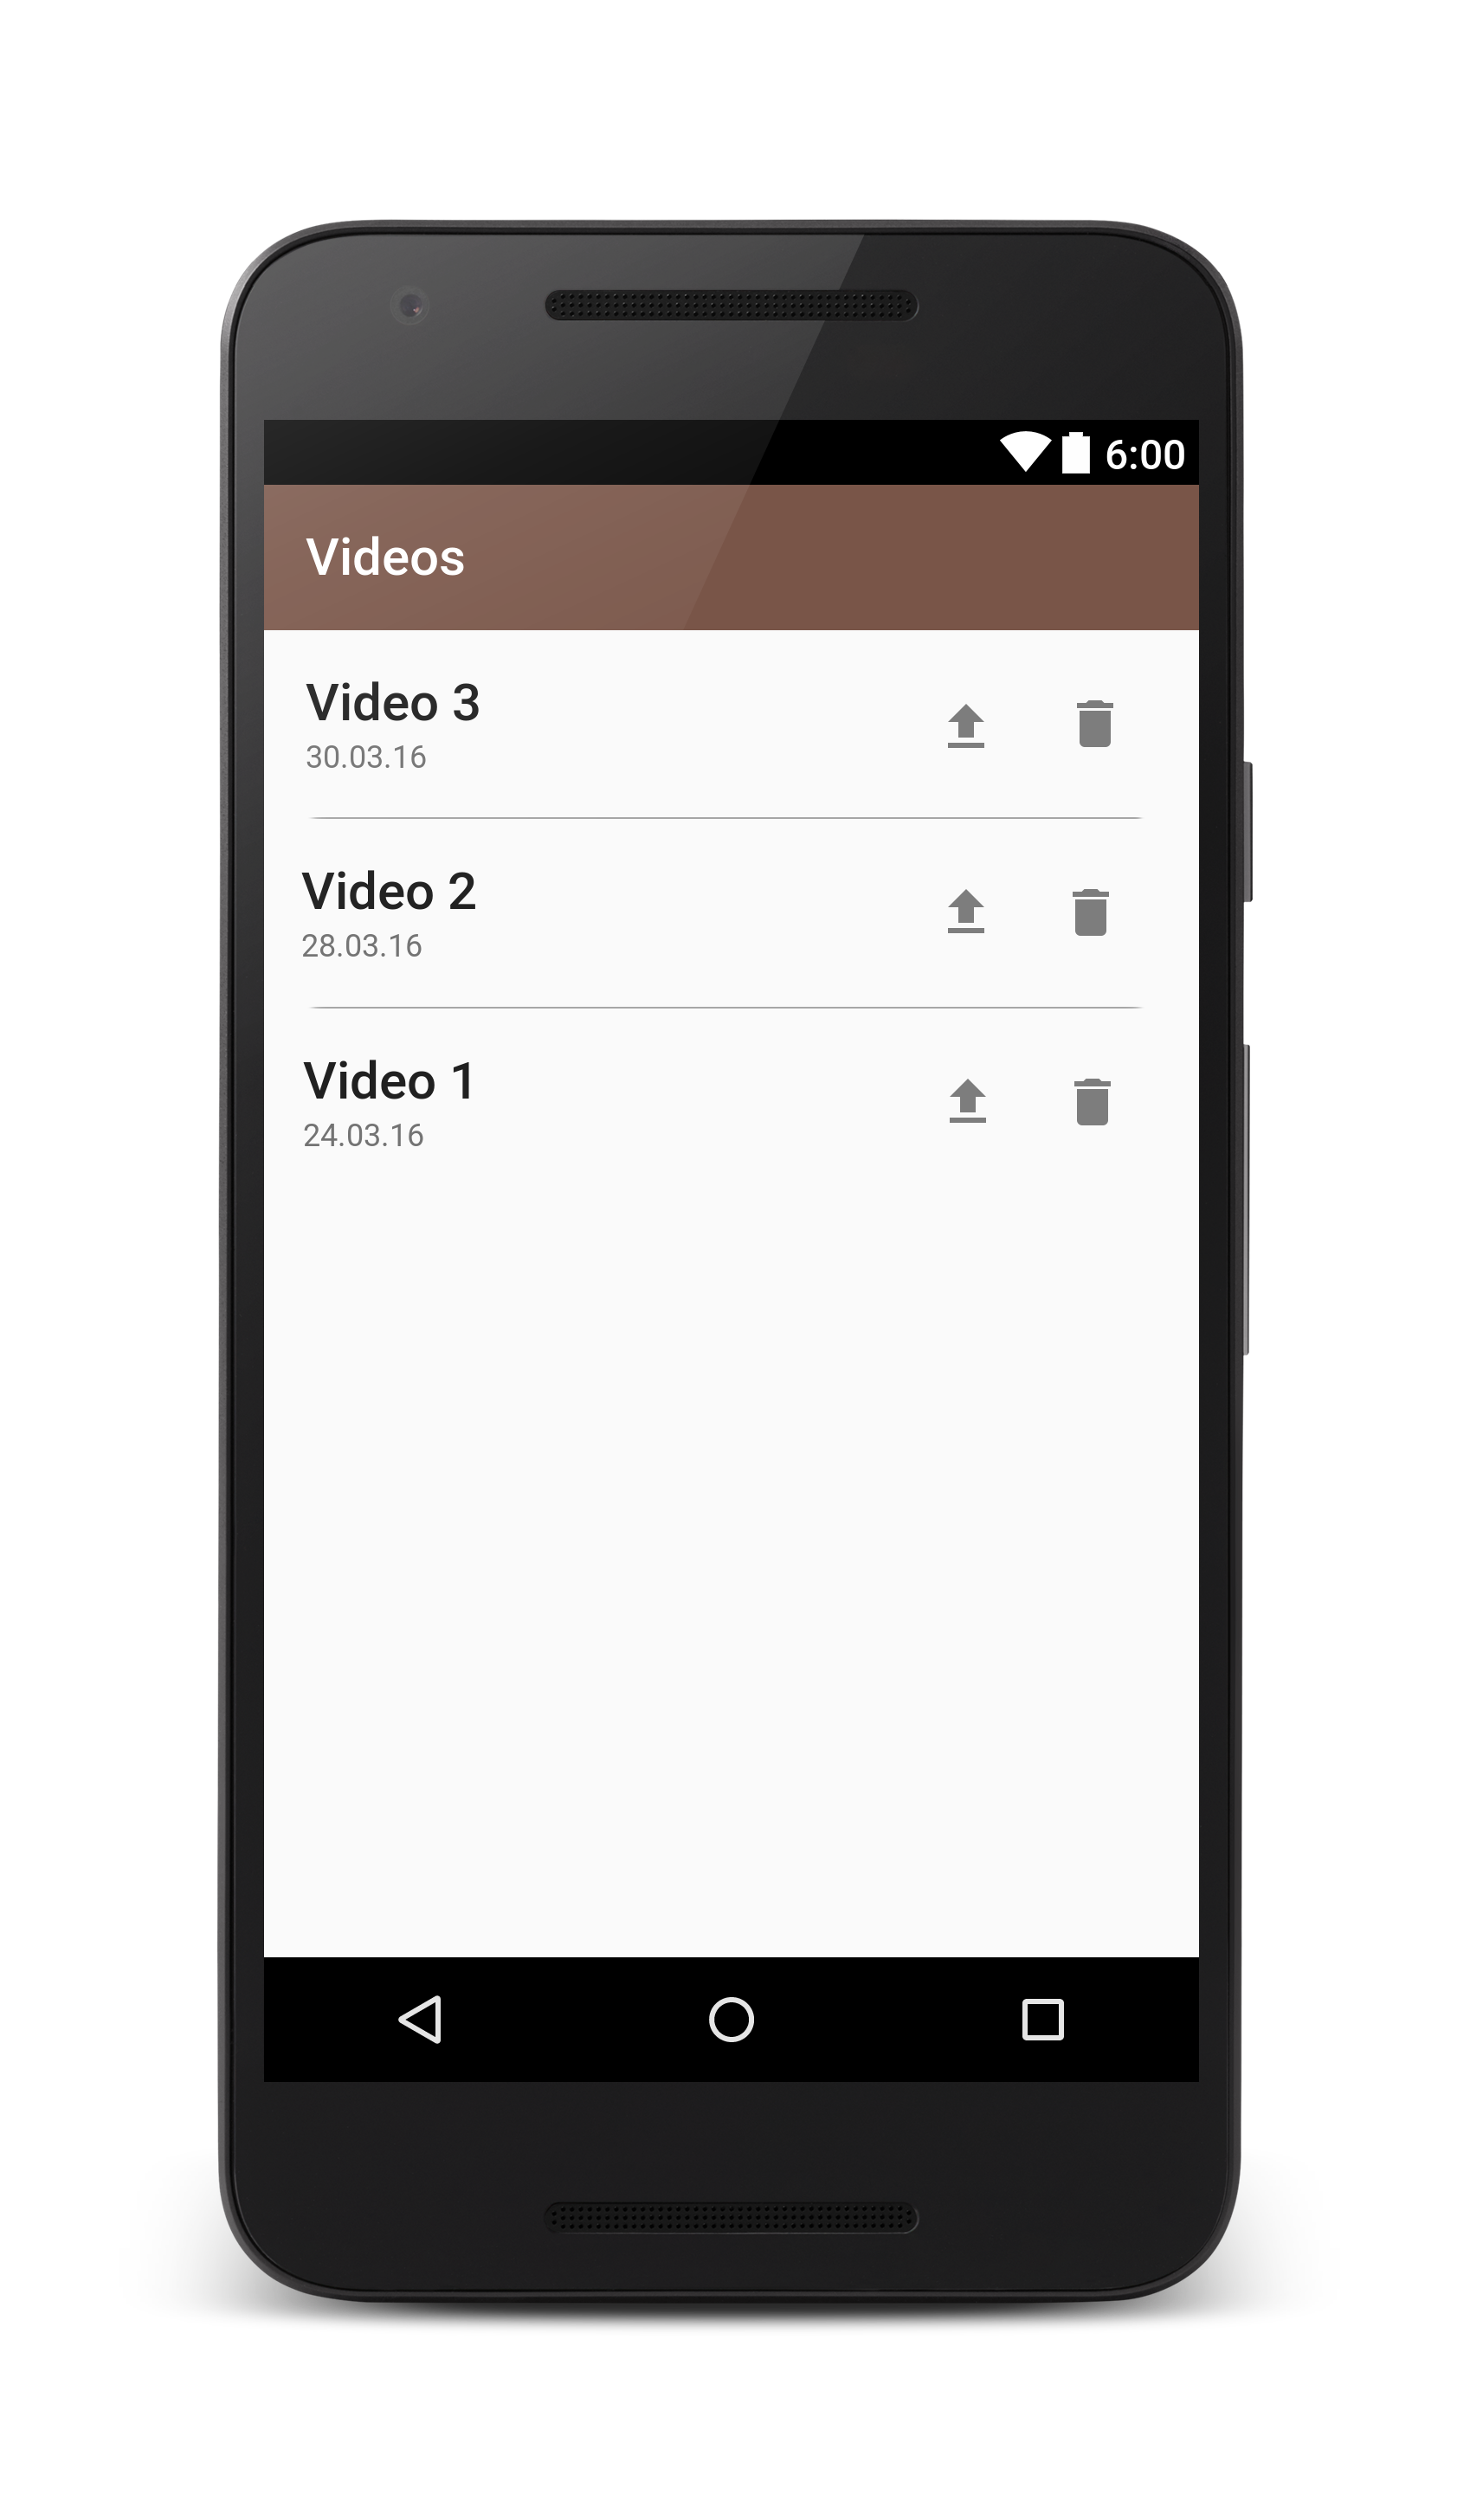
\includegraphics[width=0.4\textwidth]{subtopicsFuncspec/Res/Mockups/Videos_list1_phone.png}
  		\end{center}
  		\vspace{-20pt}
  		\vspace{-10pt}
	\end{wrapfigure}
Klickt der Benutzer lange auf ein Video, wird ein Fenster geöffnet, das dem Benutzer die Video-\gls{Metadaten} (Erstellungsdatum, Größe, Auflösung, Dauer, Auslöseart, \gls{G-Sensor}-Daten) als Dialog anzeigt. Schließt der Nutzer den Dialog, kehrt er zu der Liste seiner Videos~\eqref{fa:vidAnsicht} zurück.

\item \label{fa:einstAnsicht}\textbf{Anzeigen der Einstellungen} \hfill \\
Wählt der Benutzer im Menü die Option ``Einstellungen'', so werden dem Nutzer die Einstellungen (Auflösung, Bildwiederholrate, Größe \gls{Ringpuffer}) angezeigt. Diese sind mit Standardparametern festgelegt.

\item \label{fa:imprAnsicht}\textbf{Anzeigen rechtlicher Informationen} \hfill \\
Wählt der Benutzer im Menü die Option ``Impressum'', gelangt er zur Impressums-Ansicht. Von dort kann er sich das Impressum~\eqref{fa:imprAnzeigen} und die Datenschutzerklärung~\eqref{fa:datenschAnzeigen} anzeigen lassen.
\end{minipage}

\item \label{fa:imprAnzeigen}\textbf{Anzeigen des Impressums} \hfill \\
Wählt der Benutzer ``Impressum'' auf der Impressum-Ansicht, wird ein Dialog angezeigt, der das Impressum anzeigt.

\item \label{fa:datenschAnzeigen}\textbf{Anzeigen der Datenschutzerklärung} \hfill \\
Wählt der Benutzer ``Datenschutzerklärung'' auf der Impressum-Ansicht, wird ein Dialog angezeigt, der die Datenschutzerklärung anzeigt.

\end{enumerate}




\section{\gls{Web-Dienst}}
\begin{enumerate}
\renewcommand{\labelenumi}{\textbf{\theenumi}}
\renewcommand{\theenumi}{FA\arabic{enumi}0}
\setcounter{enumi}{199}

\item \label{fa:empfangVid} \textbf{Empfangen eines Videos von der \gls{App}} \hfill \\
Bekommt der \gls{Web-Dienst} eine Anfrage von der App, ein Video hochzuladen, so überprüft er zunächst, ob er die Anfrage bearbeiten kann, oder ob bereits zu viele andere Anfragen gestellt wurden~\eqref{na:paralleleZugriffe}. Ist dies nicht der Fall, so entschlüsselt er das Video~\eqref{fa:entschVideo} und beginnt die Anonymisierung~\eqref{fa:anonymVideo}. Bei Fehlern bei der Anfrage bzw. wenn der Server die Anfrage annimmt, beantwortet der Server die Anfrage mit einer Fehlermeldung bzw. Erfolgsmeldung.

\item  \label{fa:entschVideo}\textbf{Entschlüsseln eines empfangenen Videos} \hfill \\
Bevor der \gls{Web-Dienst} die Bearbeitung des Videos beginnt, entschlüsselt er das empfangene verschlüsselte Video ~\ref{sec:Verschlüsselung}. Das entschlüsselte Video wird lokal temporär gespeichert.

\item  \label{fa:anonymVideo}\textbf{\glslink{anonymisieren}{Anonymisierung} des Videos} \hfill \\
Der \gls{Web-Dienst} analysiert zunächst das Video~\eqref{fa:relBildbereiche}. Die dadurch gefundenen, für die Anonymisierung relevanten Bildbereiche werden mithilfe von Bildfiltern unkenntlich gemacht.

\item  \label{fa:relBildbereiche}\textbf{Identifizieren der relevanten Bildbereiche} \hfill \\
Der \gls{Web-Dienst} nimmt das entschlüsselte Video und lässt einen Bildfilter über das Video laufen, der die für die Anonymisierung relevanten Bildbereiche (Gesichter, Nummernschilder, etc.) erkennt.

\item \label{fa:speichVideo}\textbf{Abspeichern eines \glslink{anonymisieren}{anonymisierten} Videos} \hfill \\
Nachdem das Video anonymisiert wurde, wird es auf dem Server gespeichert und alle temporären Dateien werden gelöscht. Das gespeicherte Video wird zur Videoverwaltung hinzugefügt, damit es vom Benutzer eingesehen und bearbeitet werden kann. Wenn ein Benutzer die maximale Anzahl Videos pro Account~\eqref{na:VideoKap} überschreitet, wird automatisch das älteste Video des Accounts auf dem Server gelöscht.

\item \label{fa:accSpeichern}\textbf{Speichern eines Accounts} \hfill \\
Wenn ein Nutzer sich registriert~\eqref{fa:erstellAcc}, werden seine Accountdaten auf dem Server gespeichert. Passwörter werden ausschließlich als \gls{Hash-Code} abgelegt. Zusätzlich wird hinterlegt, dass der Account noch nicht verifiziert wurde.

\item \label{fa:vidHerunterladen}\textbf{Video herunterladen} \hfill \\
Möchte ein Nutzer ein anonymisiertes Video herunterladen~\eqref{fa:anonymVidherunt}, so stellt der Server die Videodaten bereit und startet das Herunterladen.

\item \label{fa:vidLöschen}\textbf{Video löschen} \hfill \\
Möchte ein Nutzer eines seiner hochgeladenen Videos löschen~\eqref{fa:anonymVidlösch}, so werden die Videodaten vom Server gelöscht.

\item \label{fa:mailSenden}\textbf{Versenden einer Bestätigungsmail} \hfill \\
Hat ein Benutzer das Anmeldeformular~\eqref{fa:erstellAcc} ausgefüllt, so versendet der \gls{Web-Dienst} eine Bestätigungsmail. Klickt der Benutzer auf den dort vorhanden Bestätigungslink, so wird der Account verifiziert.

\item \label{fa:accLöschen}\textbf{Löschen eines Accounts} \hfill \\
Wenn der Nutzer seinen Account löschen will, werden zunächst alle von ihm hochgeladenen Videos vom Server gelöscht. Wird gerade ein Video des Benutzers anonymisiert, so wird dieses nach der Anonymisierung nicht gespeichert. Danach werden die Accountdaten des Nutzers gelöscht.

\item \label{fa:accÄndern}\textbf{Accountdaten ändern} \hfill \\
Hat der Nutzer seine Accountdaten geändert~\eqref{fa:accDatBearb}, so werden die Änderungen entsprechend auf dem Server hinterlegt.

\item \label{fa:speichVideo}\textbf{Abspeichern eines \glslink{anonymisieren}{anonymisierten} Videos} \hfill \\
Nachdem das Video anonymisiert wurde, wird es lokal auf dem Server gespeichert und alle temporären Dateien gelöscht. Das gespeicherte Video wird der Videoverwaltung hinzugefügt damit es vom Benutzer eingesehen und bearbeitet werden kann. Wenn ein Benutzer die maximale Anzahl Videos pro Account ~\eqref{na:VideoKap} überschreitet, wir automatisch das älteste Video des Accounts auf dem Server gelöscht.

\item  \label{fa:fehlerbehandlung}\textbf{Fehlerbehandlung für nicht mehr existierende Daten} \hfill \\
Werden bei einer Anfrage Daten angefragt, die nicht mehr existieren, so wird ein Fehler zurückgegeben.
\end{enumerate}





\section{\gls{Web-Interface}}
\begin{enumerate}
\renewcommand{\labelenumi}{\textbf{\theenumi}}
\renewcommand{\theenumi}{FA\arabic{enumi}0}
\setcounter{enumi}{299}
\item \label{fa:loginWeb} \textbf{Anzeigen der Anmeldeansicht} \hfill \\
Ruft der Nutzer die Privacy-Crash-Cam-Webseite auf, so gelangt er zu der Anmeldeansicht. Dort kann sich der Benutzer anmelden~\eqref{fa:weblogIn} oder sich registrieren~\eqref{fa:erstellAcc}.

\item \label{fa:erstellAcc}\textbf{Erstellen eines Benutzeraccounts} \hfill \\
Klickt der Benutzer auf "'Account erstellen"' so öffnet sich der Registrierungsdialog. Dort wird der Nutzer gebeten eine \gls{E-Mail} Adresse anzugeben. Zudem muss er ein Passwort auswählen und bestätigen. Klickt der Nutzer auf "'Registrierung abschließen"',  werden die Eingaben überprüft. Schlägt dies fehl, bleibt der Benutzer in dem Registrierungsdialog. Nach dem Erstellen eines Benutzeraccounts~\eqref{fa:accSpeichern} sendet der Server eine Bestätigungsmail~\eqref{fa:mailSenden}.

\item \label{fa:weblogIn}\textbf{Anmelden auf der Webseite} \hfill \\
Zum Anmelden auf die Webseite müssen Benutzername und Passwort korrekt in die entsprechenden Felder eingetragen sein. Nur verifizierte Nutzer~\eqref{fa:mailSenden} können sich anmelden. Bei falschen Eingaben kehrt er zur Anmeldeansicht zurück und erhält eine Fehlermeldung.

\item \textbf{Anzeigen der Menüleiste} \hfill \\
Befindet sich der Nutzer in einer anderen Ansicht als der Anmeldeansicht, so befindet sich am linken Rand der Websteite die Menüleiste. Dort kann der Nutzer die Liste der \glslink{anonymisieren}{anonymisierten} Videos~\eqref{fa:anonymVidAnzeigen} in seinem Account bearbeiten~\eqref{fa:accBearb}, die Datenschutzerklärung einsehen~\eqref{fa:datenschutzWeb}, das Impressum einsehen~\eqref{fa:impressumWeb}, oder sich abmelden~\eqref{fa:weblogOut}.

\item \label{fa:anonymVidAnzeigen}\textbf{Anzeigen der Liste der \glslink{anonymisieren}{anonymisierten} Videos} \hfill \\
Hat sich ein Benutzer eingeloggt, wird er automatisch auf diese Ansicht weitergeleitet. Hier werden die, vom Nutzer hochgeladenen Videos chronologisch aufgelistet. Der Nutzer kann Videos herunterladen~\eqref{fa:anonymVidherunt}, löschen~\eqref{fa:anonymVidlösch},  oder die Videoinformationen einsehen~\eqref{fa:anonymViddaten}.

\item \label{fa:anonymVidherunt}\textbf{Herunterladen von \glslink{anonymisieren}{anonymisierten} Videos} \hfill \\
Durch einen Klick auf das ``Herunterlade-Icon'' wird ein Speicherdialog geöffnet. Nachdem der Nutzer einen Speicherort ausgewählt hat, wird das Video heruntergeladen~\eqref{fa:vidHerunterladen}. Bricht der Benutzer den Dialog ab, bleibt er in der Listenansicht seiner Videos.

\item \label{fa:anonymVidlösch}\textbf{Löschen eines \glslink{anonymisieren}{anonymisierten} Videos} \hfill \\
Durch den Klick auf das ``Löschen-Symbol'' wird ein Bestätigungsdialog geöffnet. Falls der Benutzer bestätigt, wird das Video aus der Liste seiner hochgeladenen Videos entfernt und vom Server gelöscht~\eqref{fa:vidLöschen}. Bricht der Benutzer den Dialog ab, bleibt er in der Listenansicht seiner Videos. Videos werden auch gelöscht nachdem der Nutzer mehr Videos hochgeladen hat als zulässig~\eqref{na:VideoKap} ist. Dabei wird das älteste Video zuerst gelöscht.

\item \label{fa:anonymViddaten}\textbf{Einsehen von Video-Daten der \glslink{anonymisieren}{anonymisierten} Videos} \hfill \\
Klickt der Benutzer auf das ``Info-Symbol'', so wird ein Fenster geöffnet, das dem Benutzer die Video-\gls{Metadaten} (Erstellungsdatum, Datum der Anonymisierung, Größe, Auflösung, Dauer) anzeigt.

\item \label{fa:accBearb}\textbf{Bearbeiten eines Benutzeraccounts} \hfill \\
Klickt ein Benutzer in der Menüleiste auf ``Account bearbeiten'', so wird ein Fenster geöffnet, in dem der Nutzer auswählen kann, ob er seine Accountdaten ändern oder seinen Account löschen will.

\item \label{fa:accLöschenWeb}\textbf{Account löschen} \hfill \\
Klickt der Benutzer im Fenster~\eqref{fa:accBearb} auf ``Account Löschen'', so öffnet sich ein Bestätigungsdialog, in dem der Benutzer gefragt wird, ob er wirklich seinen Account löschen will. Bestätigt dieser, so gelangt er zu der Anmeldeansicht~\eqref{fa:loginWeb} und sein Account wird gelöscht~\eqref{fa:accLöschen}.

\item \label{fa:accDatBearb}\textbf{Accountdaten bearbeiten} \hfill \\
Klickt der Benutzer in dem Fenster~\eqref{fa:accBearb} auf ``Accountdaten ändern'', so kann er sein Passwort ändern. Dies macht er, indem er zunächst in ein Feld sein altes Passwort und danach in zwei Felder sein neues gewünschtes Passwort eingibt. Stimmt das alte Passwort und stimmen die zwei Felder für das neue Passwort überein, so werden die Daten auf dem Server entsprechend geändert~\eqref{fa:accÄndern}.

\item \label{fa:impressumWeb} \textbf{Anzeigen des Impressums} \hfill \\
Klickt der Benutzer in der Menüleiste auf ``Impressum'', so wird eine Sicht geöffnet, in der der Nutzer das Impressum einsehen kann.

\item \label{fa:datenschutzWeb} \textbf{Anzeigen der Datenschutzerklärung} \hfill \\
Klickt der Benutzer in der Menüleiste auf ``Datenschutz'', so wird eine Sicht geöffnet, in der der Nutzer die Datenschutzerklärung und die AGB einsehen kann.

\item \label{fa:weblogOut}\textbf{Anmelden von der Webseite} \hfill \\
Klickt ein Benutzer in der Menüleiste auf ``Abmelden'', so wird er auf die Anmeldeansicht~\eqref{fa:loginWeb} zurückgeleitet. Schließt ein Nutzer die Webseite, so wird er automatisch ausgeloggt.

\end{enumerate}